% ============================================================================
%  অধ্যায় ৬ : স্থানাঙ্ক জ্যামিতি ১
%  COMPILE WITH XeLaTeX  (twice, so the point total resolves)
%  Overleaf: Menu -> Compiler -> XeLaTeX
%  Requires: bnhandout.sty  and  fonts/Kalpurush.ttf  in the project
% ============================================================================
\documentclass[11pt]{article}
\usepackage{bnhandout}

\usepackage{amsmath}
\usepackage{amssymb}
\usepackage{tikz}

\hauthor[https://jugantordey.github.io/]{Jugantor Dey}
\hseries{\textit{Mathematics for the Physics Olympiad}}

\begin{document}

\handouttitle{Chapter 6 : Coordinate Geometry I}

\noindent
এই অধ্যায়ে ঢোকার আগে অধ্যায় ৪ (ফাংশন ১) ও অধ্যায় ৫ (ইউক্লিডীয়
জ্যামিতি ১) শেষ করে নাও। ৪ থেকে লাগবে function, domain, range আর সেটের ভাষা;
৫ থেকে লাগবে পিথাগোরাসের উপপাদ্য, তার বিপরীত উপপাদ্য, আর সদৃশ ত্রিভুজ। বৃত্তের
অনুচ্ছেদে অধ্যায় ৩-এর বর্গ পূর্ণ করার কৌশলটিও একবার কাজে লাগবে।

অধ্যায় ৪-এ function-এর লেখচিত্র ইচ্ছে
করেই এড়িয়ে যাওয়া হয়েছিল, কারণ যে সমতলের উপর লেখচিত্র আঁকা হয় সেটাই তখনো গড়ে তোলা হয়নি। এই অধ্যায়ে সেটাই গড়া হবে।

এই অনুচ্ছেদগুলোর আসল কথাটা একটাই: স্থানাঙ্ক জ্যামিতি জ্যামিতিকে বীজগণিতে
অনুবাদ করে দেয়। ``দুটি রেখা লম্ব'' একটা জ্যামিতিক বাক্য, যা প্রমাণ করতে ছবি
আঁকতে হয়; কিন্তু $m_1 m_2 = -1$ একটা বীজগাণিতিক বাক্য, যা যাচাই করতে কেবল
গুণ করলেই চলে। এই অনুবাদটুকুই ডেকার্তে (Re(né Descartes) ও ফার্মা (Pierre de Fermat)-এর আবিষ্কার, আর পদার্থবিজ্ঞানের
প্রায় প্রতিটি হিসাব এর উপরেই দাঁড়িয়ে।

এই অধ্যায়ে মোট \totalpoints\ পয়েন্ট আছে।

% ============================================================================
\section{কার্তেসীয় সমতল}
% ============================================================================

\begin{idea}[সমতলের স্থানাঙ্ক]
সমতলের উপর দুটি লম্ব সংখ্যারেখা আঁকো, যারা একে অপরকে দুজনেরই শূন্য বিন্দুতে
কাটে। আনুভূমিকটিকে বলে $x$-অক্ষ, উল্লম্বটিকে বলে $y$-অক্ষ, আর ছেদবিন্দুটিকে
বলে origin, লেখা হয় $O$।

এখন সমতলের যেকোনো বিন্দু $P$ নাও। $P$ থেকে দুই অক্ষের উপর লম্ব ফেললে $x$-অক্ষে
একটি সংখ্যা $a$ আর $y$-অক্ষে একটি সংখ্যা $b$ পাওয়া যায়। এই দুটি সংখ্যা লিখে
রাখি ক্রমজোড় $(a, b)$ হিসেবে; $a$-কে বলে $P$-এর $x$- (ভুজ বা abscissa) আর $b$-কে বলে
$y$-coordinate (কোটি বা coordinate)।

শব্দটা ``ক্রম''জোড়, আর ক্রমটা গুরুত্বপূর্ণ: $(2, 3)$ ও $(3, 2)$ সমতলের দুটি
ভিন্ন বিন্দু।
\end{idea}

\noindent
অধ্যায় ৪-এর ভাষায় কথাটা আরও পরিষ্কার করে বলা যায়। সব ক্রমজোড়ের সেটটিকে
লেখা হয়
\[
  \mathbb{R}^2 = \{\, (a, b) : a \in \mathbb{R} \text{ এবং } b \in \mathbb{R} \,\},
\]
আর উপরের নিয়মটি সমতলের বিন্দু থেকে $\mathbb{R}^2$-এ একটি bijection তৈরি করে:
প্রতিটি বিন্দুর জন্য ঠিক একটি ক্রমজোড়, আর প্রতিটি ক্রমজোড়ের জন্য ঠিক একটি
বিন্দু। এই bijection-টাই গোটা অনুচ্ছেদের ইঞ্জিন, কারণ এর জোরেই জ্যামিতির যেকোনো
প্রশ্নকে সংখ্যার প্রশ্নে বদলে ফেলা যায়।

দুই অক্ষ মিলে সমতলটিকে চারটি অংশে ভাগ করে, যাদের বলে quadrant, আর গোনা হয়
ডান দিকের উপরেরটি থেকে শুরু করে ঘড়ির কাঁটার উল্টো দিকে।

\begin{center}
\begin{tikzpicture}[scale=0.78]
  \draw[->] (-3.6,0) -- (3.6,0) node[right] {$x$};
  \draw[->] (0,-3.0) -- (0,3.0) node[above] {$y$};
  \node[below left] at (0,0) {$O$};
  \node at (2.0,1.6) {I};
  \node at (-2.0,1.6) {II};
  \node at (-2.0,-1.6) {III};
  \node at (2.0,-1.6) {IV};
  \node at (2.0,2.35) {\small $x>0,\ y>0$};
  \node at (-2.0,2.35) {\small $x<0,\ y>0$};
  \node at (-2.0,-2.35) {\small $x<0,\ y<0$};
  \node at (2.0,-2.35) {\small $x>0,\ y<0$};
  \fill (2.5,1.0) circle (2.2pt);
  \node[above right] at (2.5,1.0) {\small $(2.5,\,1)$};
  \draw[dashed] (2.5,0) -- (2.5,1.0) -- (0,1.0);
\end{tikzpicture}
\end{center}

\begin{idea}[বক্ররেখা মানে সমাধান সেট]
$x$ ও $y$ নিয়ে একটি শর্ত লিখলে সেই শর্ত যেসব বিন্দু মানে, তারা মিলে সমতলের
একটি অংশ তৈরি করে। এই সেটটিকেই বলে ওই শর্তের সমাধান সেট, আর সমীকরণের ক্ষেত্রে
একে বলা হয় সমীকরণটির লেখচিত্র:
\[
  \{\, (x, y) \in \mathbb{R}^2 : \text{শর্তটি সত্য} \,\}.
\]
এই এক লাইনেই গোটা স্থানাঙ্ক জ্যামিতির ব্যাকরণ ধরা আছে। ``সরলরেখা'', ``বৃত্ত''
বা ``অধিবৃত্ত'' কোনো আলাদা জাতের বস্তু নয়; এরা সবাই এক জিনিস, কেবল শর্তটা
আলাদা।
\end{idea}

\begin{remark}
অধ্যায় ৪-এ $f \colon A \to B$ function-এর লেখচিত্র সংজ্ঞায়িত করার কথা
বলে রাখা হয়েছিল। এখন সেটা লিখে ফেলা যায়:
\[
  \{\, (x, f(x)) : x \in A \,\}.
\]
এটাও একটা সমাধান সেট, শর্তটি হলো $y = f(x)$। আর সেখানকার ``দোটানা চলবে না''
শর্তটির ছবি-রূপও এখন বলা যায়: কোনো উল্লম্ব রেখা এই সেটটিকে একবারের বেশি
কাটতে পারবে না, কারণ কাটলে একই $x$-এর দুটি ভিন্ন মান থাকত। একেই বলে
উল্লম্ব রেখা পরীক্ষা।
\end{remark}

\begin{example}
নিচের সেট দুটি সমতলের কোন অংশ, বর্ণনা করো।
\[
  \text{(ক)}\ \ \{\, (x,y) : x < 0 \,\}
  \qquad\qquad
  \text{(খ)}\ \ \{\, (x,y) : |y| \leq 2 \,\}
\]
\end{example}

\begin{solbox}
(ক) শর্তটি কেবল $x$-এর উপর, $y$-এর উপর কোনো শর্ত নেই। তাই $y$ যা খুশি হতে
পারে, শুধু $x$-কে ঋণাত্মক হতে হবে। এটি $y$-অক্ষের বাঁ পাশের গোটা অঞ্চল,
অক্ষটি নিজে বাদ; কারণ অক্ষের উপর $x = 0$, যা $x < 0$ মানে না।

(খ) অধ্যায় ৪ থেকে জানি $|y| \leq 2$ মানে $-2 \leq y \leq 2$। তাই এটি
$y = -2$ ও $y = 2$ আনুভূমিক রেখা দুটির মাঝের ফালি, আর এবার রেখা দুটিও
ভেতরে আছে, কারণ শর্তে সমান চিহ্ন আছে।
\end{solbox}

% ============================================================================
\section{দূরত্ব ও মধ্যবিন্দু}
% ============================================================================

\begin{idea}[দূরত্ব]
$P_1(x_1, y_1)$ ও $P_2(x_2, y_2)$ দুটি বিন্দুর মধ্যকার দূরত্ব
\[
  |P_1 P_2| \;=\; \sqrt{(x_2 - x_1)^2 + (y_2 - y_1)^2}\,.
\]
\end{idea}

\noindent
\textbf{উৎপত্তি।} $P_3(x_2, y_1)$ বিন্দুটি নাও: এর $x$-coordinate $P_2$-এর
মতো, আর $y$-coordinate $P_1$-এর মতো। তাহলে $P_1 P_3$ আনুভূমিক এবং $P_2 P_3$
উল্লম্ব, ফলে $P_3$-এ কোণটি সমকোণ।

একই আনুভূমিক রেখার উপর দুটি বিন্দুর দূরত্ব তাদের $x$-coordinate-এর পার্থক্যের
পরম মান, তাই $|P_1 P_3| = |x_2 - x_1|$। একইভাবে $|P_2 P_3| = |y_2 - y_1|$।
এবার সমকোণী ত্রিভুজ $P_1 P_3 P_2$-তে পিথাগোরাস (অধ্যায় ৫) প্রয়োগ করে
\[
  |P_1 P_2|^2 = |x_2 - x_1|^2 + |y_2 - y_1|^2 = (x_2 - x_1)^2 + (y_2 - y_1)^2 ,
\]
কারণ যেকোনো বাস্তব $a$-এর জন্য $|a|^2 = a^2$। দূরত্ব অঋণাত্মক, তাই ধনাত্মক
বর্গমূল নিয়েই কাজ শেষ।

$x_1 = x_2$ বা $y_1 = y_2$ হলে ত্রিভুজটি চ্যাপ্টা হয়ে যায়, ফলে উপরের যুক্তি
আর খাটে না। তবে তখন সূত্রটি সরাসরি মিলিয়ে দেখা যায়: $x_1 = x_2$ হলে সূত্র দেয়
$\sqrt{(y_2-y_1)^2} = |y_2 - y_1|$, যা উল্লম্ব রেখার উপর দুটি বিন্দুর দূরত্ব
হিসেবে ঠিকই আছে। $\blacksquare$

\begin{center}
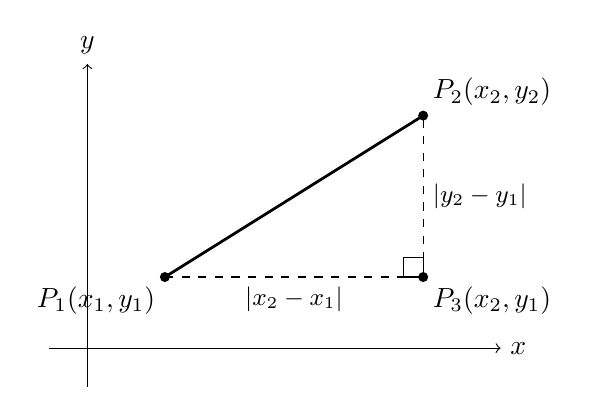
\begin{tikzpicture}[scale=0.82]
  \draw[->] (-0.6,0) -- (6.4,0) node[right] {$x$};
  \draw[->] (0,-0.6) -- (0,4.4) node[above] {$y$};
  \coordinate (P1) at (1.2,1.1);
  \coordinate (P2) at (5.2,3.6);
  \coordinate (P3) at (5.2,1.1);
  \draw[dashed] (P1) -- (P3);
  \draw[dashed] (P3) -- (P2);
  \draw[line width=1pt] (P1) -- (P2);
  \fill (P1) circle (2.2pt) node[below left] {$P_1(x_1,y_1)$};
  \fill (P2) circle (2.2pt) node[above right] {$P_2(x_2,y_2)$};
  \fill (P3) circle (2.2pt) node[below right] {$P_3(x_2,y_1)$};
  \node[below] at (3.2,1.1) {\small $|x_2-x_1|$};
  \node[right] at (5.2,2.35) {\small $|y_2-y_1|$};
  \draw (4.9,1.1) rectangle (5.2,1.4);
\end{tikzpicture}
\end{center}

\begin{example}
$(2, -1)$ ও $(7, 11)$ বিন্দু দুটির দূরত্ব বের করো।
\end{example}

\begin{solbox}
\[
  d = \sqrt{(7-2)^2 + \big(11 - (-1)\big)^2} = \sqrt{5^2 + 12^2}
    = \sqrt{25 + 144} = \sqrt{169} = 13 .
\]
বিয়োগ কোন দিক থেকে করলে তা অবান্তর, কারণ পরে বর্গ করা হচ্ছে:
$(2-7)^2$ আর $(7-2)^2$ একই।
\end{solbox}

\begin{idea}[মধ্যবিন্দু]
$P_1(x_1, y_1)$ ও $P_2(x_2, y_2)$ রেখাংশটির মধ্যবিন্দু
\[
  M \;=\; \left( \frac{x_1 + x_2}{2},\ \frac{y_1 + y_2}{2} \right).
\]
অর্থাৎ দুই প্রান্তের coordinate-গুলোর গড়।
\end{idea}

\noindent
\textbf{উৎপত্তি।} উপরের $M$ ধরে দূরত্ব সূত্র দিয়ে হিসাব করি:
\[
  |P_1 M|^2 = \left( \frac{x_1+x_2}{2} - x_1 \right)^2
            + \left( \frac{y_1+y_2}{2} - y_1 \right)^2
            = \frac{(x_2-x_1)^2 + (y_2-y_1)^2}{4} ,
\]
\[
  |M P_2|^2 = \left( x_2 - \frac{x_1+x_2}{2} \right)^2
            + \left( y_2 - \frac{y_1+y_2}{2} \right)^2
            = \frac{(x_2-x_1)^2 + (y_2-y_1)^2}{4} .
\]
দুটি সমান, এবং দুটিই $|P_1P_2|^2 / 4$। বর্গমূল নিয়ে পাই
\[
  |P_1 M| = |M P_2| = \tfrac{1}{2} |P_1 P_2| .
\]
তাই $M$ দুই প্রান্ত থেকে সমদূরবর্তী, আর দূরত্বদুটি মিলে গোটা রেখাংশের দৈর্ঘ্য
হয়। $M$ যে সত্যিই রেখাংশটির উপরেই পড়ে, সেটা ঢাল দিয়ে দেখা যায়; ওটা সমস্যা ৩-এ
তোমার জন্য রাখা হলো। $\blacksquare$

% ============================================================================
\section{ঢাল}
% ============================================================================

\begin{idea}[ঢাল]
কোনো অ-উল্লম্ব সরলরেখার উপর $P_1(x_1, y_1)$ ও $P_2(x_2, y_2)$ দুটি ভিন্ন
বিন্দু হলে রেখাটির ঢাল (slope)
\[
  m \;=\; \frac{\Delta y}{\Delta x} \;=\; \frac{y_2 - y_1}{x_2 - x_1}\,.
\]
লব হলো উল্লম্ব পরিবর্তন বা rise, হর হলো আনুভূমিক পরিবর্তন বা run।

উল্লম্ব রেখার ঢাল সংজ্ঞায়িত নয়, কারণ তখন $x_1 = x_2$ হয়ে হর শূন্য হয়ে যায়।
লক্ষ করো, এটা ``ঢাল অসীম'' নয়; এটা ``ঢাল বলে কিছু নেই''।
\end{idea}

\begin{center}
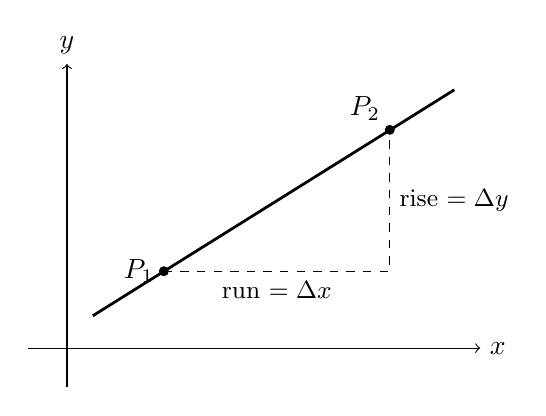
\begin{tikzpicture}[scale=0.82]
  \draw[->] (-0.6,0) -- (6.4,0) node[right] {$x$};
  \draw[->] (0,-0.6) -- (0,4.4) node[above] {$y$};
  \draw[line width=1pt] (0.4,0.5) -- (6.0,4.0);
  \coordinate (A) at (1.5,1.19);
  \coordinate (B) at (5.0,3.38);
  \coordinate (C) at (5.0,1.19);
  \draw[dashed] (A) -- (C) -- (B);
  \fill (A) circle (2.2pt) node[left] {$P_1$};
  \fill (B) circle (2.2pt) node[above left] {$P_2$};
  \node[below] at (3.25,1.19) {\small run $= \Delta x$};
  \node[right] at (5.0,2.28) {\small rise $= \Delta y$};
\end{tikzpicture}
\end{center}

\begin{idea}[ঢাল কোন দুটি বিন্দু নিলে তার উপর নির্ভর করে না]
একই রেখার উপর ভিন্ন ভিন্ন জোড়া বিন্দু নিলেও উপরের ভগ্নাংশটির মান একই থাকে।
তাই ``রেখাটির ঢাল'' কথাটা অর্থপূর্ণ।
\end{idea}

\noindent
\textbf{প্রমাণ।} ধরি একই রেখার উপর দুই জোড়া বিন্দু $P_1, P_2$ এবং $Q_1, Q_2$,
কোনোটিই উল্লম্বভাবে সাজানো নয়। আগের ছবির মতো দুই জোড়ার জন্য দুটি সমকোণী
ত্রিভুজ আঁকো, যাদের একটি বাহু আনুভূমিক আর একটি উল্লম্ব।

দুই ত্রিভুজেরই এক কোণ সমকোণ। আর দুটিরই অতিভুজ একই সরলরেখার অংশ, আর একটি
করে বাহু $x$-অক্ষের সমান্তরাল; তাই ওই রেখা ছেদক হিসেবে যে অনুরূপ কোণ তৈরি
করে, সেটি দুই ত্রিভুজে সমান। দুটি কোণ সমান হলেই ত্রিভুজদুটি সদৃশ
(অধ্যায় ৫)।

সদৃশ ত্রিভুজে অনুরূপ বাহুর অনুপাত সমান, তাই
\[
  \frac{\text{উল্লম্ব বাহু}}{\text{আনুভূমিক বাহু}}
\]
দুই ত্রিভুজে সমান। চিহ্নও মেলে, কারণ একই রেখা বরাবর ডান দিকে গেলে $y$ হয়
দুবারই বাড়ে, নয়তো দুবারই কমে। সুতরাং দুই জোড়া বিন্দু একই ঢাল দেয়।
$\blacksquare$

\begin{example}
$(-2, 5)$ ও $(4, -7)$ বিন্দু দিয়ে যাওয়া রেখার ঢাল বের করো।
\end{example}

\begin{solbox}
\[
  m = \frac{-7 - 5}{4 - (-2)} = \frac{-12}{6} = -2 .
\]
ঋণাত্মক ঢাল, তাই ডান দিকে এগোলে রেখাটি নামে। মানটির মানে হলো: $x$ এক একক
বাড়লে $y$ দুই একক কমে।
\end{solbox}

\begin{idea}[ঢাল হলো পরিবর্তনের হার]
$m = \Delta y / \Delta x$ ভগ্নাংশটিকে কেবল ``খাড়াভাব'' না ভেবে আরেকভাবে পড়া
যায়: $x$ এক একক বাড়লে $y$ কত বাড়ে। অর্থাৎ ঢাল হলো $x$-এর সাপেক্ষে $y$-এর
পরিবর্তনের হার (rate of change)।

সরলরেখার বেলায় এই হারটি সর্বত্র এক। বস্তুত ``রেখাটি সরল'' কথাটার বীজগাণিতিক
মানেই তাই: হারটি বদলায় না।
\end{idea}

\begin{remark}
এই দ্বিতীয় পাঠটাই এই গোটা সিরিজের সবচেয়ে গুরুত্বপূর্ণ একটি সূত্র, তাই এখানে
থামা যাক।

সময়ের সাপেক্ষে অবস্থানের লেখচিত্র আঁকলে ঢাল হয় বেগ; বেগের লেখচিত্রে ঢাল হয়
ত্বরণ। কিন্তু বাস্তবে গতি খুব কমই সুষম, তাই লেখচিত্রও খুব কমই সরলরেখা।
বাঁকা লেখচিত্রে $\Delta y / \Delta x$ নির্ভর করে তুমি কোন দুটি বিন্দু নিচ্ছ
তার উপর, ফলে ``ঢাল'' কথাটার আর একটিমাত্র মানে থাকে না।

সমাধানটা হলো দুটি বিন্দুকে ক্রমশ কাছাকাছি এনে ওই অনুপাতটির limit নেওয়া। সেই
limit-এর নাম derivative, আর সেটা আসবে অধ্যায় ১৫  -তে। আজ যা শিখছ, সেটা তার
প্রথম বীজ: derivative আসলে ঢাল ছাড়া আর কিছুই নয়, কেবল একটিমাত্র বিন্দুতে
মাপা।
\end{remark}

% ============================================================================
\section{সরলরেখা}
% ============================================================================

\begin{idea}[বিন্দু-ঢাল রূপ]
$P_1(x_1, y_1)$ বিন্দু দিয়ে যাওয়া, $m$ ঢালবিশিষ্ট রেখাটির সমীকরণ
\[
  y - y_1 = m (x - x_1).
\]
\end{idea}

\noindent
\textbf{উৎপত্তি।} $P(x,y)$ বিন্দুটি, যেখানে $x \neq x_1$, ওই রেখার উপর
থাকবে তখনই যখন $P_1 P$ রেখাংশের ঢাল $m$-এর সমান, অর্থাৎ
\[
  \frac{y - y_1}{x - x_1} = m .
\]
দুই পাশে $(x - x_1)$ দিয়ে গুণ করলে $y - y_1 = m(x - x_1)$। গুণটি বৈধ, কারণ
$x \neq x_1$। আর $x = x_1, y = y_1$ বসালেও সমীকরণটি $0 = 0$ হয়ে সত্য থাকে,
তাই $P_1$ নিজেও এর সমাধান সেটে আছে। সুতরাং সমাধান সেটটি ঠিক রেখাটিই।
$\blacksquare$

\begin{idea}[ঢাল-ছেদক রূপ ও সাধারণ রূপ]
যে রেখা $y$-অক্ষকে $(0, b)$ বিন্দুতে কাটে এবং যার ঢাল $m$, তার সমীকরণ
বিন্দু-ঢাল রূপে $y - b = m(x - 0)$, অর্থাৎ
\[
  y = mx + b .
\]
এখানে $b$-কে বলে $y$-intercept। একইভাবে রেখাটি $x$-অক্ষকে যেখানে কাটে, সেই
$x$-মানটিকে বলে $x$-intercept।

আবার যেকোনো রেখাকেই লেখা যায়
\[
  Ax + By + C = 0
\]
আকারে, যেখানে $A$ ও $B$ একসঙ্গে শূন্য নয়। অ-উল্লম্ব রেখার জন্য
$y = mx + b$ থেকে $-mx + y - b = 0$ নিলেই হয়; আর উল্লম্ব রেখার সমীকরণ
$x = a$, অর্থাৎ $x - a = 0$। এই তৃতীয় রূপটির সুবিধা হলো উল্লম্ব রেখাও এর
মধ্যে ধরা পড়ে।
\end{idea}

\begin{example}
$(-2, 1)$ ও $(4, -5)$ বিন্দু দিয়ে যাওয়া রেখার সমীকরণ বের করো, এবং তার দুটি
intercept বের করো।
\end{example}

\begin{solbox}
প্রথমে ঢাল:
\[
  m = \frac{-5 - 1}{4 - (-2)} = \frac{-6}{6} = -1 .
\]
$(-2, 1)$ বিন্দু ধরে বিন্দু-ঢাল রূপে
\[
  y - 1 = -1\,(x + 2) \ \Longrightarrow\ y = -x - 1 .
\]
$y$-intercept হলো $-1$। $x$-intercept পেতে $y = 0$ বসাই: $0 = -x - 1$,
অর্থাৎ $x = -1$।

যাচাই করে নেওয়া ভালো: $(4, -5)$ বসালে $-4 - 1 = -5$, মিলে গেছে।
\end{solbox}

\begin{idea}[সমান্তরালের শর্ত]
দুটি ভিন্ন অ-উল্লম্ব রেখা সমান্তরাল হবে তখনই, যখন তাদের ঢাল সমান।
\end{idea}

\noindent
\textbf{প্রমাণ।} রেখা দুটি $y = m_1 x + b_1$ ও $y = m_2 x + b_2$। ``সমান্তরাল''
মানে এদের কোনো সাধারণ বিন্দু নেই। সাধারণ বিন্দু থাকা মানে এমন $x$ থাকা যার
জন্য
\[
  m_1 x + b_1 = m_2 x + b_2 ,
  \qquad \text{অর্থাৎ} \qquad
  (m_1 - m_2)\,x = b_2 - b_1 .
\]
এটি অধ্যায় ২-এর চেনা সরল সমীকরণ, আর তার তিনটি সম্ভাবনা:

$m_1 \neq m_2$ হলে হর শূন্য নয়, তাই $x = \dfrac{b_2 - b_1}{m_1 - m_2}$ একটিমাত্র
সমাধান আছে; রেখা দুটি ঠিক একবার মিলিত হয়, সমান্তরাল নয়।

$m_1 = m_2$ ও $b_1 \neq b_2$ হলে সমীকরণটি দাঁড়ায় $0 = b_2 - b_1 \neq 0$, যা
কখনো সত্য নয়; কোনো সাধারণ বিন্দু নেই, তাই সমান্তরাল।

$m_1 = m_2$ ও $b_1 = b_2$ হলে সব $x$-ই সমাধান; রেখা দুটি আসলে একই রেখা, তাই
``ভিন্ন'' শর্তটি বাদ পড়ে।

সুতরাং ভিন্ন দুটি অ-উল্লম্ব রেখা সমান্তরাল হবে ঠিক তখনই যখন $m_1 = m_2$।
$\blacksquare$

\begin{idea}[লম্বের শর্ত]
দুটি অ-উল্লম্ব রেখা পরস্পর লম্ব হবে তখনই, যখন
\[
  m_1 m_2 = -1 , \qquad \text{অর্থাৎ} \qquad m_2 = -\frac{1}{m_1}\,.
\]
\end{idea}

\noindent
\textbf{প্রমাণ।} লম্ব হতে হলে রেখা দুটিকে মিলিত হতেই হবে; ধরি তারা $P$ বিন্দুতে
মেলে। প্রথম রেখার উপর $P$ থেকে ডান দিকে ঠিক এক একক সরে যে বিন্দুটি পাই তাকে
বলি $A$, আর দ্বিতীয় রেখার উপর একইভাবে পাওয়া বিন্দুটিকে বলি $B$। ঢালের
সংজ্ঞা অনুযায়ী $A$ হলো $P$ থেকে ডানে $1$ ও উপরে $m_1$, আর $B$ হলো $P$ থেকে
ডানে $1$ ও উপরে $m_2$।

দূরত্ব সূত্র দিয়ে তিনটি দৈর্ঘ্যের বর্গ বের করি। $A$ ও $B$ দুজনেরই
$x$-coordinate $P$-এর চেয়ে $1$ বেশি, তাই তাদের মধ্যে আনুভূমিক পার্থক্য শূন্য:
\[
  |PA|^2 = 1 + m_1^2 , \qquad
  |PB|^2 = 1 + m_2^2 , \qquad
  |AB|^2 = (m_2 - m_1)^2 .
\]
অধ্যায় ৫ অনুযায়ী $P$-এ কোণটি সমকোণ হবে তখনই, যখন
$|PA|^2 + |PB|^2 = |AB|^2$; এক দিকে পিথাগোরাস, উল্টো দিকে তার বিপরীত উপপাদ্য।
শর্তটি লিখি:
\[
  (1 + m_1^2) + (1 + m_2^2) = m_2^2 - 2 m_1 m_2 + m_1^2 .
\]
দুই পাশ থেকে $m_1^2 + m_2^2$ কাটলে থাকে
\[
  2 = -2 m_1 m_2 , \qquad \text{অর্থাৎ} \qquad m_1 m_2 = -1 .
\]
প্রতিটি ধাপ উভমুখী, তাই শর্তটি ঠিক লম্ব হওয়ার সমতুল্য।

একটি রেখা উল্লম্ব হলে এই হিসাব খাটে না, কারণ তখন ঢালই নেই। সে ক্ষেত্রে অন্য
রেখাটিকে আনুভূমিক হতে হবে, অর্থাৎ তার ঢাল $0$; আর $m_1 m_2 = -1$ শর্তটি তখন
অর্থহীন। $\blacksquare$

\begin{center}
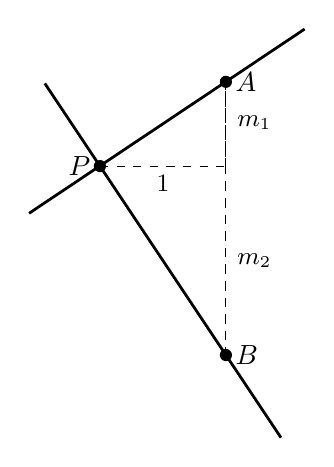
\begin{tikzpicture}[scale=1.0]
  \coordinate (P) at (0,0);
  \coordinate (A) at (1.6,1.07);
  \coordinate (B) at (1.6,-2.4);
  \draw[line width=1pt] (-0.9,-0.6) -- (2.6,1.74);
  \draw[line width=1pt] (-0.7,1.05) -- (2.3,-3.45);
  \draw[dashed] (P) -- (1.6,0);
  \draw[dashed] (1.6,0) -- (A);
  \draw[dashed] (1.6,0) -- (B);
  \draw[dashed] (A) -- (B);
  \fill (P) circle (2.2pt) node[left] {$P$};
  \fill (A) circle (2.2pt) node[right] {$A$};
  \fill (B) circle (2.2pt) node[right] {$B$};
  \node[below] at (0.8,0) {\small $1$};
  \node[right] at (1.62,0.55) {\small $m_1$};
  \node[right] at (1.62,-1.2) {\small $m_2$};
\end{tikzpicture}
\end{center}

\noindent
ছবিতে $m_2$ ঋণাত্মক, তাই $B$ নিচে নেমে গেছে; হিসাবে চিহ্নটি আপনা থেকেই ঠিক
জায়গায় বসে।

\begin{example}
$(3, -1)$ বিন্দু দিয়ে যাওয়া, $2x + 5y = 7$ রেখাটির (ক) সমান্তরাল এবং
(খ) লম্ব রেখার সমীকরণ বের করো।
\end{example}

\begin{solbox}
দেওয়া রেখাটিকে ঢাল-ছেদক রূপে আনি:
\[
  5y = -2x + 7 \ \Longrightarrow\ y = -\tfrac{2}{5} x + \tfrac{7}{5},
\]
তাই এর ঢাল $-\tfrac{2}{5}$।

(ক) সমান্তরাল রেখার ঢালও $-\tfrac{2}{5}$। বিন্দু-ঢাল রূপে
\[
  y + 1 = -\tfrac{2}{5}(x - 3)
  \ \Longrightarrow\ 5y + 5 = -2x + 6
  \ \Longrightarrow\ 2x + 5y - 1 = 0 .
\]

(খ) লম্ব রেখার ঢাল $m$ হলে $-\tfrac{2}{5} \cdot m = -1$, অর্থাৎ
$m = \tfrac{5}{2}$। তাই
\[
  y + 1 = \tfrac{5}{2}(x - 3)
  \ \Longrightarrow\ 2y + 2 = 5x - 15
  \ \Longrightarrow\ 5x - 2y - 17 = 0 .
\]
দুটোতেই $(3,-1)$ বসিয়ে যাচাই করে নাও।
\end{solbox}

% ============================================================================
\section{বৃত্ত}
% ============================================================================

\begin{idea}[বৃত্তের সমীকরণ]
বৃত্ত হলো একটি নির্দিষ্ট বিন্দু থেকে নির্দিষ্ট দূরত্বে থাকা সব বিন্দুর সেট।
বিন্দুটির নাম কেন্দ্র, দূরত্বটির নাম ব্যাসার্ধ।

কেন্দ্র $(h, k)$ ও ব্যাসার্ধ $r > 0$ হলে বৃত্তটির সমীকরণ
\[
  (x - h)^2 + (y - k)^2 = r^2 .
\]
কেন্দ্র origin হলে এটি দাঁড়ায় $x^2 + y^2 = r^2$।
\end{idea}

\noindent
\textbf{উৎপত্তি।} সংজ্ঞাটি বীজগণিতে অনুবাদ করলেই হয়ে গেল। $P(x,y)$ বৃত্তের
উপর থাকবে তখনই, যখন কেন্দ্র $C(h,k)$ থেকে তার দূরত্ব ঠিক $r$:
\[
  \sqrt{(x-h)^2 + (y-k)^2} = r .
\]
দুই পাশ অঋণাত্মক, তাই বর্গ করলে সমাধান সেট বদলায় না, এবং পাই
$(x-h)^2 + (y-k)^2 = r^2$। $\blacksquare$

\begin{remark}
লক্ষ করো, বৃত্ত এখানে আকাশ থেকে পড়েনি। প্রথম অনুচ্ছেদের ধারণাটি ছিল ``বক্ররেখা
মানে সমাধান সেট'', আর দ্বিতীয় অনুচ্ছেদে দূরত্বকে সংখ্যায় প্রকাশ করা হয়েছিল।
এই দুটো হাতে থাকলে বৃত্তের সমীকরণ আর আলাদা করে মুখস্থ করার জিনিস নয়; এটা দুই
লাইনের হিসাব।
\end{remark}

\begin{example}
কেন্দ্র $(-3, 4)$ ও ব্যাসার্ধ $5$ বিশিষ্ট বৃত্তের সমীকরণ লেখো।
\end{example}

\begin{solbox}
$h = -3$, $k = 4$, $r = 5$ বসিয়ে
\[
  (x + 3)^2 + (y - 4)^2 = 25 .
\]
লক্ষ করো $h$ ঋণাত্মক বলে বন্ধনীর ভেতরে যোগ চিহ্ন এসেছে। এই জায়গাটাতেই সবচেয়ে
বেশি ভুল হয়।
\end{solbox}

\begin{example}
$x^2 + y^2 - 4x + 10y + 20 = 0$ সমীকরণটি একটি বৃত্ত নির্দেশ করে; তার কেন্দ্র ও
ব্যাসার্ধ বের করো।
\end{example}

\begin{solbox}
$x$-এর পদগুলো একসঙ্গে আর $y$-এর পদগুলো একসঙ্গে সাজাই, ধ্রুবকটি ডান পাশে
পাঠিয়ে:
\[
  (x^2 - 4x) + (y^2 + 10y) = -20 .
\]
এবার অধ্যায় ৩-এর কৌশলে দুই বন্ধনীতেই বর্গ পূর্ণ করি, অর্থাৎ $x$-এর
সহগের অর্ধেকের বর্গ $\left(\tfrac{-4}{2}\right)^2 = 4$ আর $y$-এর জন্য
$\left(\tfrac{10}{2}\right)^2 = 25$ দুই পাশেই যোগ করি:
\[
  (x^2 - 4x + 4) + (y^2 + 10y + 25) = -20 + 4 + 25 ,
\]
\[
  (x - 2)^2 + (y + 5)^2 = 9 .
\]
তুলনা করে পাই কেন্দ্র $(2, -5)$ এবং $r^2 = 9$, অর্থাৎ ব্যাসার্ধ $3$।
\end{solbox}

\begin{remark}
$x^2 + y^2 + Dx + Ey + F = 0$ আকারের প্রতিটি সমীকরণ কিন্তু বৃত্ত নয়। বর্গ
পূর্ণ করার পর ডান পাশে যে সংখ্যাটি পড়ে, সেটিই ঠিক করে দেয় কী পাওয়া গেল:

ডান পাশ ধনাত্মক হলে সেটি একটি বৃত্ত।

ডান পাশ শূন্য হলে সমাধান সেটে কেবল কেন্দ্রটিই থাকে, কারণ দুটি বর্গের যোগফল
শূন্য হয় তখনই যখন দুটিই শূন্য। একটিমাত্র বিন্দু, বৃত্ত নয়।

ডান পাশ ঋণাত্মক হলে কোনো সমাধানই নেই, কারণ বাস্তব সংখ্যার বর্গ ঋণাত্মক হয় না।
সমাধান সেট ফাঁকা।

উদাহরণ: উপরের সমীকরণে $20$-এর জায়গায় $30$ বসালে ডান পাশ দাঁড়ায় $-1$, আর
সমতলে একটিও বিন্দু থাকে না।
\end{remark}

% ============================================================================
\section{সমস্যা}
% ============================================================================

\prob{1} নিচের বিন্দু-জোড়াগুলোর দূরত্ব বের করো।
\begin{enumerate}
  \item $(2, -1)$ ও $(7, 11)$
  \item $(a, b)$ ও $(b, a)$
\end{enumerate}

\begin{sol}
\begin{enumerate}
  \item $\sqrt{5^2 + 12^2} = \sqrt{169} = 13$.
  \item
        \[
          \sqrt{(b-a)^2 + (a-b)^2} = \sqrt{2(a-b)^2} = |a - b|\sqrt{2}\,.
        \]
        পরম মান লাগবেই, কারণ $a < b$ হলে $a - b$ ঋণাত্মক, অথচ দূরত্ব
        কখনো ঋণাত্মক নয়।
\end{enumerate}
\end{sol}

\prob{1} নিচের রেখাংশগুলোর মধ্যবিন্দু বের করো।
\begin{enumerate}
  \item $(1, 3)$ ও $(7, 15)$
  \item $(-4, 2)$ ও $(6, -8)$
\end{enumerate}

\begin{sol}
\begin{enumerate}
  \item $\left( \dfrac{1+7}{2}, \dfrac{3+15}{2} \right) = (4, 9)$.
  \item $\left( \dfrac{-4+6}{2}, \dfrac{2-8}{2} \right) = (1, -3)$.
\end{enumerate}
\end{sol}

\prob{2} $P_1(x_1, y_1)$ ও $P_2(x_2, y_2)$ দুটি বিন্দু, যেখানে
$x_1 \neq x_2$, আর $M$ হলো তাদের মধ্যবিন্দু। ঢাল ব্যবহার করে দেখাও যে
$P_1$, $M$, $P_2$ একই সরলরেখার উপর আছে।

\begin{sol}
$M = \left( \dfrac{x_1+x_2}{2}, \dfrac{y_1+y_2}{2} \right)$ ধরে $P_1M$-এর ঢাল
বের করি:
\[
  \frac{\frac{y_1+y_2}{2} - y_1}{\frac{x_1+x_2}{2} - x_1}
  = \frac{\frac{y_2-y_1}{2}}{\frac{x_2-x_1}{2}}
  = \frac{y_2 - y_1}{x_2 - x_1}\,.
\]
এবার $MP_2$-এর ঢাল:
\[
  \frac{y_2 - \frac{y_1+y_2}{2}}{x_2 - \frac{x_1+x_2}{2}}
  = \frac{\frac{y_2-y_1}{2}}{\frac{x_2-x_1}{2}}
  = \frac{y_2 - y_1}{x_2 - x_1}\,.
\]
দুটি ঢাল সমান, আর রেখাংশ দুটির একটি সাধারণ বিন্দু $M$ আছে। একই বিন্দু দিয়ে
যাওয়া সমান ঢালের দুটি রেখা একই রেখা, তাই তিনটি বিন্দুই সমরেখ।

হর শূন্য হওয়ার আশঙ্কা নেই, কারণ $x_1 \neq x_2$ ধরা আছে। $x_1 = x_2$ হলে
তিনটি বিন্দুরই $x$-coordinate এক, তাই তারা একটি উল্লম্ব রেখার উপর থাকে।
\end{sol}

\prob{2} দেখাও যে $(0, 3)$, $(-4, 0)$ ও $(4, 0)$ শীর্ষবিশিষ্ট ত্রিভুজটি
সমদ্বিবাহু।

\begin{sol}
শীর্ষ তিনটিকে $A(0,3)$, $B(-4,0)$, $C(4,0)$ বলি।
\[
  |AB| = \sqrt{(-4-0)^2 + (0-3)^2} = \sqrt{16+9} = 5 ,
\]
\[
  |AC| = \sqrt{(4-0)^2 + (0-3)^2} = \sqrt{16+9} = 5 ,
\]
\[
  |BC| = \sqrt{(4+4)^2 + 0^2} = 8 .
\]
$|AB| = |AC| = 5$, তাই ত্রিভুজটি সমদ্বিবাহু। সমকোণী নয়, কারণ
$5^2 + 5^2 = 50 \neq 64 = 8^2$.
\end{sol}

\prob{2} $(-2, 1)$ ও $(4, -5)$ বিন্দু দিয়ে যাওয়া রেখার সমীকরণ ঢাল-ছেদক রূপে
লেখো, এবং তার $x$-intercept ও $y$-intercept বের করো।

\begin{sol}
ঢাল $m = \dfrac{-5-1}{4+2} = -1$। $(-2,1)$ ধরে
\[
  y - 1 = -(x + 2) \ \Longrightarrow\ y = -x - 1 .
\]
$x = 0$ বসিয়ে $y$-intercept $= -1$; $y = 0$ বসিয়ে $x$-intercept $= -1$।
\end{sol}

\prob{3} $(3, -1)$ বিন্দু দিয়ে যাওয়া, $2x + 5y = 7$ রেখাটির লম্ব রেখার
সমীকরণ বের করো। এরপর দুটি রেখার ছেদবিন্দু বের করো, এবং $(3,-1)$ থেকে দেওয়া
রেখাটির দূরত্ব বের করো।

\begin{sol}
দেওয়া রেখার ঢাল $-\tfrac{2}{5}$, তাই লম্ব রেখার ঢাল $\tfrac{5}{2}$:
\[
  y + 1 = \tfrac{5}{2}(x - 3) \ \Longrightarrow\ 5x - 2y - 17 = 0 .
\]
ছেদবিন্দুর জন্য $2x + 5y = 7$ ও $5x - 2y = 17$ সমাধান করি। প্রথমটিকে $2$ দিয়ে
আর দ্বিতীয়টিকে $5$ দিয়ে গুণ করে যোগ করলে
\[
  4x + 10y = 14, \qquad 25x - 10y = 85
  \ \Longrightarrow\ 29x = 99 .
\]
সুতরাং $x = \tfrac{99}{29}$, আর $2x + 5y = 7$ থেকে
\[
  5y = 7 - \tfrac{198}{29} = \tfrac{203 - 198}{29} = \tfrac{5}{29},
  \qquad y = \tfrac{1}{29}.
\]
ছেদবিন্দু $\left( \tfrac{99}{29}, \tfrac{1}{29} \right)$।

লম্ব দূরত্ব হলো $(3,-1)$ থেকে এই ছেদবিন্দুর দূরত্ব:
\[
  \Delta x = \tfrac{99}{29} - 3 = \tfrac{12}{29}, \qquad
  \Delta y = \tfrac{1}{29} + 1 = \tfrac{30}{29},
\]
\[
  d = \frac{1}{29}\sqrt{12^2 + 30^2} = \frac{\sqrt{144 + 900}}{29}
    = \frac{\sqrt{1044}}{29} = \frac{6\sqrt{29}}{29} = \frac{6}{\sqrt{29}}\,.
\]
\end{sol}

\prob{3} $A(2, 1)$, $B(6, 4)$, $C(-1, 5)$ ত্রিভুজটি সমকোণী।
\begin{enumerate}
  \item পিথাগোরাসের বিপরীত উপপাদ্য ব্যবহার করে তা দেখাও।
  \item ঢাল ব্যবহার করে আবার তা দেখাও।
  \item ত্রিভুজটির ক্ষেত্রফল বের করো।
\end{enumerate}

\begin{sol}
\begin{enumerate}
  \item
        \[
          |AB|^2 = 4^2 + 3^2 = 25, \quad
          |AC|^2 = (-3)^2 + 4^2 = 25, \quad
          |BC|^2 = (-7)^2 + 1^2 = 50 .
        \]
        যেহেতু $|AB|^2 + |AC|^2 = 25 + 25 = 50 = |BC|^2$, বিপরীত উপপাদ্য
        অনুযায়ী $A$-তে কোণটি সমকোণ।
  \item $AB$-এর ঢাল $\dfrac{4-1}{6-2} = \dfrac{3}{4}$, আর $AC$-এর ঢাল
        $\dfrac{5-1}{-1-2} = -\dfrac{4}{3}$। গুণফল
        $\dfrac{3}{4} \cdot \left(-\dfrac{4}{3}\right) = -1$, তাই
        $AB \perp AC$।
  \item সমকোণ $A$-তে, তাই $AB$ ও $AC$ হলো দুই বাহু, দুটিরই দৈর্ঘ্য $5$:
        \[
          \text{ক্ষেত্রফল} = \tfrac{1}{2} \cdot 5 \cdot 5 = \tfrac{25}{2} .
        \]
\end{enumerate}
\end{sol}

\prob{3} নিচের প্রতিটি সমীকরণের সমাধান সেট কী, নির্ণয় করো।
\begin{enumerate}
  \item $x^2 + y^2 - 4x + 10y + 20 = 0$
  \item $x^2 + y^2 - 4x + 10y + 29 = 0$
  \item $x^2 + y^2 - 4x + 10y + 30 = 0$
\end{enumerate}

\begin{sol}
তিনটিতেই বর্গ পূর্ণ করার কাজ এক, কেবল ধ্রুবকটি আলাদা। সব ক্ষেত্রেই
\[
  (x - 2)^2 + (y + 5)^2 = 29 - F ,
\]
যেখানে $F$ হলো ধ্রুবক পদটি; কারণ $4 + 25 = 29$।

\begin{enumerate}
  \item $F = 20$, তাই ডান পাশ $9$। এটি $(2, -5)$ কেন্দ্রবিশিষ্ট $3$
        ব্যাসার্ধের বৃত্ত।
  \item $F = 29$, তাই ডান পাশ $0$। দুটি বর্গের যোগফল শূন্য হলে দুটিই শূন্য,
        অর্থাৎ $x = 2$ ও $y = -5$। সমাধান সেটে একটিমাত্র বিন্দু $(2,-5)$;
        এটি বৃত্ত নয়।
  \item $F = 30$, তাই ডান পাশ $-1$। বাস্তব সংখ্যার বর্গ অঋণাত্মক, তাই বাঁ
        পাশ কখনো ঋণাত্মক হতে পারে না। সমাধান সেট ফাঁকা।
\end{enumerate}
\end{sol}

\prob{3} $y$-অক্ষের উপর এমন একটি বিন্দু বের করো, যা $(5, -5)$ ও $(1, 1)$
থেকে সমদূরবর্তী।

\begin{sol}
$y$-অক্ষের উপরের বিন্দু মানে $x$-coordinate শূন্য, তাই বিন্দুটি $(0, y)$।
বর্গমূল এড়াতে দূরত্বের বর্গ নিয়েই কাজ করি:
\[
  (0-5)^2 + (y+5)^2 = (0-1)^2 + (y-1)^2 ,
\]
\[
  25 + y^2 + 10y + 25 = 1 + y^2 - 2y + 1 .
\]
$y^2$ দুই পাশ থেকে কাটে, থাকে
\[
  50 + 10y = 2 - 2y \ \Longrightarrow\ 12y = -48 \ \Longrightarrow\ y = -4 .
\]
বিন্দুটি $(0, -4)$। যাচাই: $(5,-5)$ থেকে দূরত্ব $\sqrt{25 + 1} = \sqrt{26}$,
আর $(1,1)$ থেকে $\sqrt{1 + 25} = \sqrt{26}$। মিলে গেছে।
\end{sol}

\prob{3} $x^2 + y^2 - 6x - 8y = 0$ বৃত্তটি নিয়ে কাজ করো।
\begin{enumerate}
  \item কেন্দ্র ও ব্যাসার্ধ বের করো।
  \item দেখাও যে এটি origin দিয়ে যায়।
  \item এটি $x$-অক্ষ ও $y$-অক্ষকে কোথায় কাটে?
  \item $(1, 1)$ বিন্দুটি বৃত্তের ভেতরে না বাইরে?
\end{enumerate}

\begin{sol}
\begin{enumerate}
  \item বর্গ পূর্ণ করে
        \[
          (x^2 - 6x + 9) + (y^2 - 8y + 16) = 0 + 9 + 16
          \ \Longrightarrow\ (x-3)^2 + (y-4)^2 = 25 .
        \]
        কেন্দ্র $(3, 4)$, ব্যাসার্ধ $5$।
  \item মূল সমীকরণে $x = 0, y = 0$ বসালে বাঁ পাশ শূন্য, ডান পাশও শূন্য।
        তাই origin বৃত্তের উপর আছে। (কেন্দ্র থেকে origin-এর দূরত্ব
        $\sqrt{9+16} = 5$, যা ঠিক ব্যাসার্ধ।)
  \item $y = 0$ বসিয়ে $x^2 - 6x = 0$, অর্থাৎ $x(x-6) = 0$, তাই $x = 0$ ও
        $x = 6$। $x$-অক্ষকে কাটে $(0,0)$ ও $(6,0)$ বিন্দুতে।

        $x = 0$ বসিয়ে $y^2 - 8y = 0$, অর্থাৎ $y = 0$ ও $y = 8$। $y$-অক্ষকে
        কাটে $(0,0)$ ও $(0,8)$ বিন্দুতে।
  \item কেন্দ্র থেকে $(1,1)$-এর দূরত্ব
        \[
          \sqrt{(1-3)^2 + (1-4)^2} = \sqrt{4 + 9} = \sqrt{13} .
        \]
        $\sqrt{13} < 5$, তাই বিন্দুটি বৃত্তের ভেতরে।
\end{enumerate}
\end{sol}

\prob{3} $A(-1, 3)$ ও $B(5, -1)$ থেকে সমদূরবর্তী সব বিন্দুর সেটটির সমীকরণ
বের করো, এবং দেখাও যে এটি $AB$ রেখাংশের লম্ব সমদ্বিখণ্ডক।

\begin{sol}
$P(x,y)$ সমদূরবর্তী হওয়ার শর্ত, দূরত্বের বর্গ নিয়ে:
\[
  (x+1)^2 + (y-3)^2 = (x-5)^2 + (y+1)^2 .
\]
দুই পাশ খুলে লিখি:
\[
  x^2 + 2x + 1 + y^2 - 6y + 9 = x^2 - 10x + 25 + y^2 + 2y + 1 .
\]
$x^2$ ও $y^2$ কেটে যায়, থাকে
\[
  2x - 6y + 10 = -10x + 2y + 26
  \ \Longrightarrow\ 12x - 8y - 16 = 0
  \ \Longrightarrow\ 3x - 2y - 4 = 0 .
\]
এটি একটি সরলরেখা। এবার দুটি জিনিস যাচাই করি।

$AB$-এর মধ্যবিন্দু $\left( \tfrac{-1+5}{2}, \tfrac{3-1}{2} \right) = (2, 1)$,
আর $3(2) - 2(1) - 4 = 0$; তাই মধ্যবিন্দুটি রেখাটির উপর আছে।

$AB$-এর ঢাল $\dfrac{-1-3}{5+1} = -\dfrac{2}{3}$, আর $3x - 2y - 4 = 0$ রেখার
ঢাল $\dfrac{3}{2}$। গুণফল $-1$, তাই রেখাটি $AB$-এর উপর লম্ব।

মধ্যবিন্দু দিয়ে যায় এবং লম্ব, সুতরাং এটি $AB$-এর লম্ব সমদ্বিখণ্ডক।
\end{sol}

\prob{4} $A(x_1, y_1)$, $B(x_2, y_2)$, $C(x_3, y_3)$ একটি ত্রিভুজের তিন
শীর্ষ। ত্রিভুজের মধ্যমা হলো এক শীর্ষ থেকে বিপরীত বাহুর মধ্যবিন্দু পর্যন্ত
টানা রেখাংশ। প্রমাণ করো যে তিনটি মধ্যমাই
\[
  G = \left( \frac{x_1 + x_2 + x_3}{3},\ \frac{y_1 + y_2 + y_3}{3} \right)
\]
বিন্দুটি দিয়ে যায়। (এই $G$-কে বলে ত্রিভুজটির ভরকেন্দ্র।)

\begin{sol}
কৌশলটা হলো: $G$-কে আগেই লিখে ফেলে কেবল যাচাই করা যে সে প্রতিটি মধ্যমার উপর
আছে। তিনটি মধ্যমার জন্য আলাদা হিসাব করার দরকার নেই, কারণ $G$-এর সূত্রটি তিন
শীর্ষের ব্যাপারে প্রতিসম; একটির জন্য দেখাতে পারলে বাকি দুটির জন্য কেবল
নামগুলো অদলবদল করলেই হবে।

$A$ থেকে টানা মধ্যমাটি ধরি। $BC$-এর মধ্যবিন্দু
\[
  M = \left( \frac{x_2 + x_3}{2},\ \frac{y_2 + y_3}{2} \right).
\]
এখন $A$, $G$, $M$ সমরেখ কি না দেখতে হবে। $A$ থেকে দুটি বিন্দুর সরণ বের করি:
\[
  G - A = \left( \frac{x_1+x_2+x_3}{3} - x_1,\ \frac{y_1+y_2+y_3}{3} - y_1 \right)
        = \left( \frac{x_2 + x_3 - 2x_1}{3},\ \frac{y_2 + y_3 - 2y_1}{3} \right),
\]
\[
  M - A = \left( \frac{x_2+x_3}{2} - x_1,\ \frac{y_2+y_3}{2} - y_1 \right)
        = \left( \frac{x_2 + x_3 - 2x_1}{2},\ \frac{y_2 + y_3 - 2y_1}{2} \right).
\]
লিখি $p = x_2 + x_3 - 2x_1$ এবং $q = y_2 + y_3 - 2y_1$। তাহলে $A$ থেকে $G$-এর
সরণ $\left( \tfrac{p}{3}, \tfrac{q}{3} \right)$ আর $A$ থেকে $M$-এর সরণ
$\left( \tfrac{p}{2}, \tfrac{q}{2} \right)$।

ধরি $p \neq 0$। তখন $AG$-এর ঢাল
\[
  \frac{q/3}{p/3} = \frac{q}{p},
\]
আর $AM$-এর ঢাল
\[
  \frac{q/2}{p/2} = \frac{q}{p}.
\]
দুটি সমান, আর দুটি রেখাংশেরই একটি সাধারণ প্রান্ত $A$। তাই $A$, $G$, $M$
সমরেখ, অর্থাৎ $G$ ওই মধ্যমাটির উপর আছে।

$p = 0$ হলে ঢাল সংজ্ঞায়িত নয়, তাই আলাদা করে দেখি। $p = 0$ মানে
$x_2 + x_3 = 2x_1$, ফলে
\[
  G_x = \frac{x_1 + x_2 + x_3}{3} = \frac{x_1 + 2x_1}{3} = x_1,
  \qquad
  M_x = \frac{x_2+x_3}{2} = x_1 .
\]
অর্থাৎ $A$, $G$, $M$ তিনটিরই $x$-coordinate $x_1$, তাই তারা একই উল্লম্ব
রেখার উপর; এবারও সমরেখ।

সুতরাং $G$ সবসময়ই $A$ থেকে টানা মধ্যমার উপর আছে। এখন $G$-এর সংজ্ঞায়
$x_1, x_2, x_3$ ভূমিকা বদল করলে সূত্রটি হুবহু একই থাকে, তাই ঠিক একই যুক্তি
$B$ ও $C$ থেকে টানা মধ্যমা দুটির জন্যও খাটে। তিনটি মধ্যমাই $G$ দিয়ে যায়।
$\blacksquare$

উপরের হিসাবে বাড়তি একটা তথ্যও ধরা পড়েছে: $A$ থেকে $G$-এর সরণ $A$ থেকে
$M$-এর সরণের ঠিক $\tfrac{2}{3}$ গুণ, কারণ
$\left( \tfrac{p}{3}, \tfrac{q}{3} \right) = \tfrac{2}{3}
\left( \tfrac{p}{2}, \tfrac{q}{2} \right)$। অর্থাৎ ভরকেন্দ্র প্রতিটি মধ্যমাকে
শীর্ষের দিক থেকে $2 : 1$ অনুপাতে ভাগ করে।
\end{sol}

\end{document}
